%
\documentclass[11pt]{article}
\usepackage[a4paper, margin=1in
]{geometry}
\usepackage{graphicx}
\usepackage{xcolor}
\usepackage{kpfonts}
\usepackage{fancyhdr}
\usepackage[
  style=ieee,
]{biblatex}
% use package for referencing figures
\usepackage{caption}
\usepackage{subcaption}
\usepackage[capitalise]{cleveref}

\usepackage[skip=1em]{parskip}

\pagestyle{fancy}

\title{\vspace{-2em}\small{Analysis of Week 12's Paper}\\\LARGE{Chromosal Organization through Loop Extrusion}\vspace{-1em}}
\author{Minghang Li}
\date{\vspace{-1em}}

\fancyhf{}
\lhead{Current Topics in Biophysics}
\rhead{\today}

\cfoot{\thepage}

\setlength{\parindent}{0ex}

\bibliography{report}

% -- end preamble --

\begin{document}

\maketitle \thispagestyle{fancy}

\bigskip
\hrule \vspace{1pt}
\hrule height 1pt
\bigskip

% the most important part it to explain

%  + what the general question is that is being addressed. that will include some general context on chromosome conformations and chromatin accessibility. (DONE!)
%  + how we learn about chromatin conformations (Hi-C etc) (DONE!)
%  * a discussion of the author's approach, the model, and the results.
%  * what the strength and weaknesses of the model are, what is left unexplained
%  * What could be done next? What has been done since?

% This discussion will include answers to many of the questions we discussed. You'll usually include some figures from the paper to make your point.

\begin{abstract}
  Week 12's lecture discussed the paper by Fudenberg et. al., titled by "\textit{Formation of Chromosomal Domains by Loop Extrusion}". It investigated the underlying mechanism of the formation of one of the most common and important chromosomal structure -- Topologically Associating Domains (TADs). It proposed the hypothesis that TADs are formed by loop extrusion regulated by CCCTC-binding factors (CTCFs) and Loop Elongation Factors (LEFs) and tested the hypothesis through rigorous modelling and simulation.
\end{abstract}

\section{Background Introduction}

The genetic information stored in DNA sequences is not presented in a linear manner, but is rather folded and organized into three-dimensional (3D) structures, thereby allowing remotely located genomic elements interact with each other. To understand the 3D spatial genome organization better, various techniques have been developed over the years. Beyond the conventional microscopy observation that uncovered some basic principles about genome microscopy, the development of chromosome conformation capture (3C) technologies has also produced many important insights into the chromatin structure \cite{denker_second_2016}.

The 3C technology was first introduced in 2002 by Dekker et. al. originally in the hope of studying the folding of yeast chromosome \cite{dekker_capturing_2002}. It quickly inspired the emergence of an abundance of 3C-derived genomics methods. \cref{fig:3C} shows an overview of the 3C-derived technologies, which all start with the same steps. First, the DNA is crosslinked using a fixative agent, most often formaldehyde, to preserve the 3D representation of the genome. Second, the crosslinked DNA is digested with restriction enzymes to generate DNA fragments of a certain size. The DNA fragments are then ligated to specific adapters and amplified by PCR. The amplified DNA fragments are then sequenced and the sequence information is used to infer the spatial relationship between the captured DNA fragments \cite{wit_decade_2012}. Amongst all the 3C-derived technologies, Hi-C is probably the most widely used one. In Hi-C, the restriction ends of DNA fragments are filled in with biotin labeled nucleotides before the ligation step. Following a blunt ligation (usually by T4 DNA ligase), the biotin-labeled DNA fragments are purified and then captured by streptavidin-coated magnetic beads. After biotin-pulldown, the fragments are sheared into reads and then mapped back to the reference genome to generate a contact map, which is then used to score and infer the 3D structure of the genome \cite{wit_decade_2012}. Biotin pull-down and paired-end sequencing enables the detection of ligation junctions, and Next Generation Sequencing (NGS) methods makes such "all versus all" detection at a genome-wide scale possible.

% insert figure 1
\begin{figure}[htbp]
  \centering
  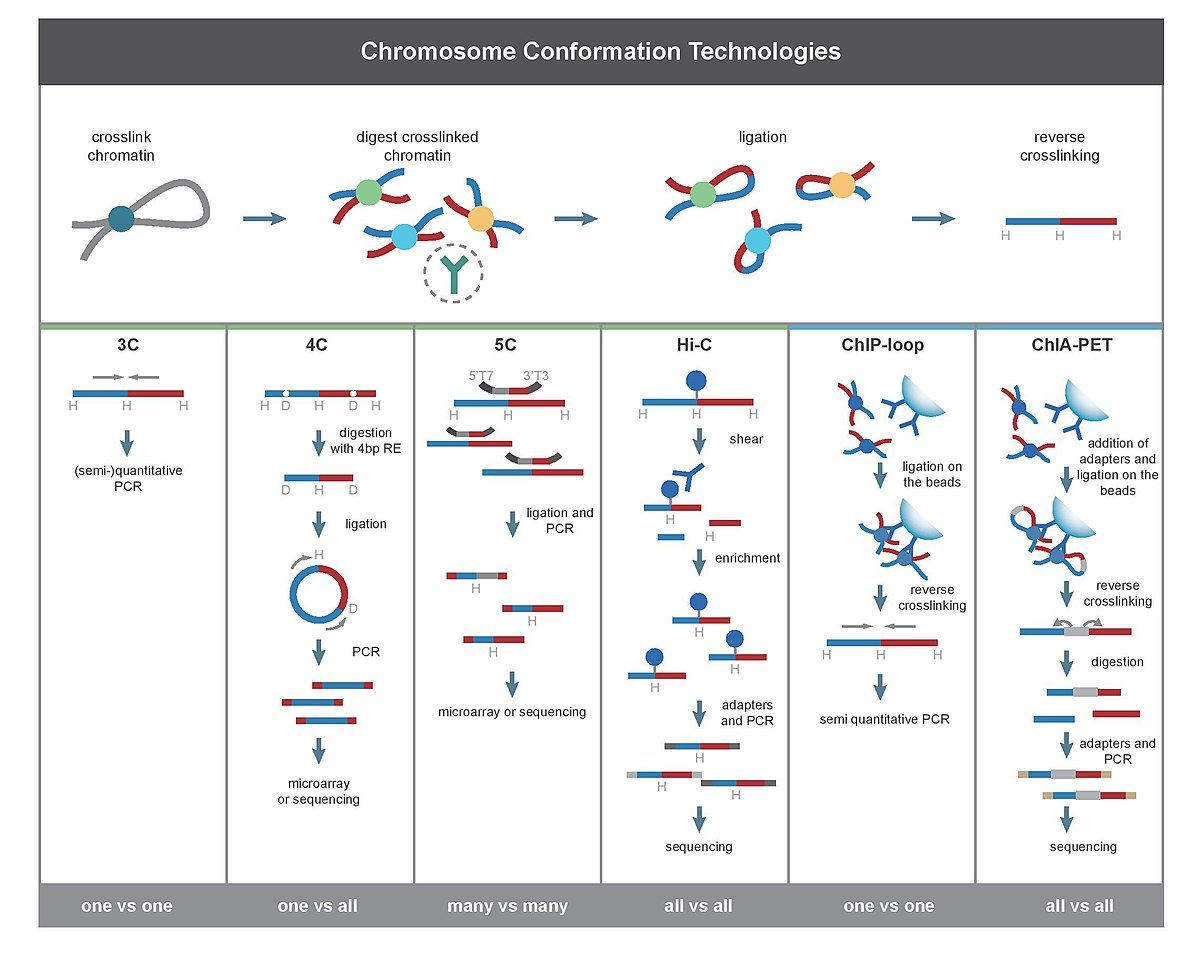
\includegraphics[width=0.8\textwidth]{assets/20221212064821.png}
  \caption{\textbf{An Overview of the 3C Technologies.}This figure comes from \cite{li_chromatin_2014}, which was adapted from \cite{wit_decade_2012}}
  \label{fig:3C}
\end{figure}

Hi-C is capable of capturing the 3D structure of the genome at a resolution of kb level. In the Hi-C contact maps, two major classes of patterns are most evident. The first one is the A/B compartmentalization which shows checkerboard-like patterns \cite{mirny_two_2019}. The A compartment is usually gene-rich, transcriptionally active and accessible (characterized by DNase I sensitivity), and the B compartment is usually the heterochromatin region that is low in expression andahs repressive histone marks \cite{denker_second_2016}\cite{wit_decade_2012}. The second one is the Topologically Associating Domains (TADs) which are characterized as continuous regions of mildly (2-4 fold) higher contact frequency than between loci in neighboring TADs \cite{mirny_two_2019}. They usually reside within a single contiguous compartment and don't necessarily exhibit the characteristic "checkerboard" pattern as A/B compartment does \cite{fudenberg_formation_2016}. 50\% of TADs have peaks of interactions at their boundaries, and they are capable of forming dynamic boundaries \cite{rao_3d_2014}. Up until the publishing of this paper, the formation of TADs was still not well understood. Previous works have proposed TADs forming mechanism based on similar monomer attraction \cite{jost_modeling_2014} and supercoiling \cite{benedetti_models_2014}, yet they fail to explain the formation of TADs in a satisfactory manner.

% by the presence of a large number of intra-TAD contacts and a low number of inter-TAD contacts. TADs are the most common and important chromosomal structure. They are usually defined as a set of genomic loci that are in close proximity to each other and are connected by a large number of intra-TAD contacts. The TADs are usually separated by a large number of inter-TAD contacts. The TADs are also usually associated with the presence of specific transcription factors and are often associated with the presence of specific gene expression patterns \cite{denker_second_2016}.
% which is sufficient to capture the large-scale organization of the genome. However, it is not capable of capturing the finer details of the genome organization. To address this issue, the authors of the paper proposed a new method called Hi-C-Pro \cite{li_chromatin_2014}. Hi-C-Pro is a Hi-C method that is capable of capturing the 3D structure of the genome at a resolution of 5 kb. It is based on the same principle as Hi-C, but with a few modifications. First, the restriction enzyme used is MboI, which cuts the DNA at a frequency of 1 kb. Second, the ligation step is performed in a two-step process. In the first step, the DNA fragments are ligated to specific adapters and amplified by PCR. In the second step, the amplified DNA fragments are ligated to a second set of adapters and amplified by PCR again. The amplified DNA fragments are then sequenced and the sequence information is used to infer the spatial relationship between the captured DNA fragments \cite{li_chromatin_2014}.

\section{Brief Summary of the Paper}

\section{Strengths and Weaknesses of the Paper}

\section{Future Prospectives}

% Bibliography
\printbibliography

\end{document}
